\chapter{Wi-Fi configuration and wiring}
Wi-Fi is normally off during ordinary operation. Because of the small antenna, keep the phone approximately 10--20~cm from the indicator during configuration.

\begin{enumerate}
\item With USB disconnected, turn on ignition or the intended vehicle supply.
\item Immediately press the rear button. The display should show a QR code.
\item Disable mobile data on the phone. Scan the QR code and connect to the indicator's Wi-Fi network. The documented default password is \texttt{1234567890}.
\item Open \url{http://192.168.4.1} on the connected phone or computer.
\item Select the application and matching sensor, save, then cycle ignition to restart.
\end{enumerate}
If the dashboard is unavailable, move closer and check that the phone remains connected to the indicator's network, even though that network has no Internet access. Retry entering QR-code mode after cycling power.

\begin{figure}[H]
\centering
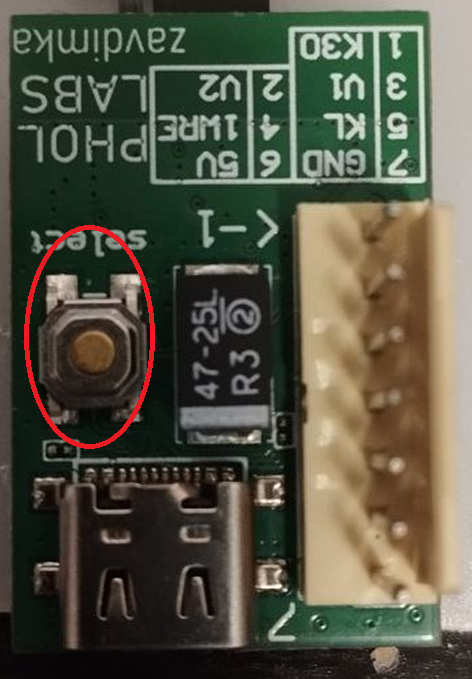
\includegraphics[width=.85\textwidth,height=.60\textheight,keepaspectratio]{figures/ivevo/image11.png}
\caption{IV-Evo reference illustration}
\end{figure}
Rear Wi-Fi boot-mode button.

\section{Common pinout}
\begin{figure}[H]
\centering
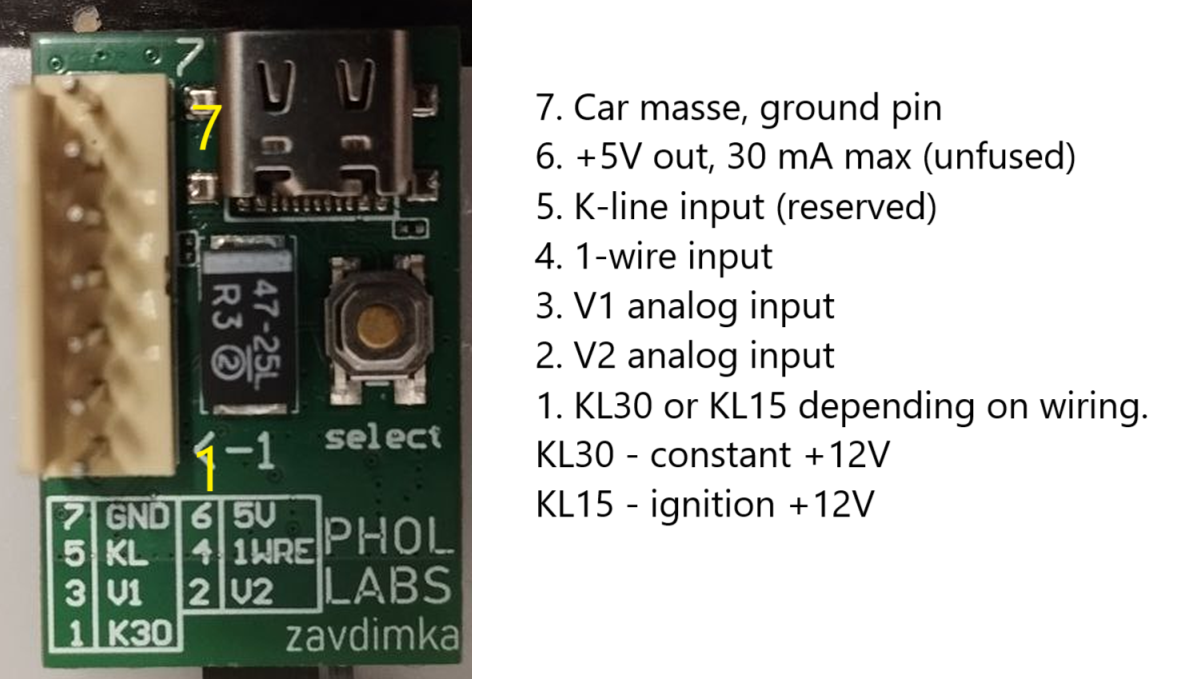
\includegraphics[width=.85\textwidth,height=.60\textheight,keepaspectratio]{figures/ivevo/image20.png}
\caption{Common pinout}
\end{figure}
The device has a seven-pin KF2510 connector. Viewed as in the photograph, the board markings are:
\begin{center}\begin{tabular}{cl}
Pin & Board marking\\\hline
1 & K30 (KL30 power input)\\
2 & V2\\
3 & V1\\
4 & 1WRE (one-wire)\\
5 & KL (K-line, reserved)\\
6 & 5V (+5 V output, 30 mA maximum)\\
7 & GND\\
\end{tabular}\end{center}
Use the numbered pins and the appropriate diagram, not wire colours alone. The supplied voltmeter diagram identifies pin 5 as reserved K-line and specifies a 30 mA maximum for the +5 V output. General analogue input voltage limits are not specified; do not infer them from the pin labels.

USB is intended for initial flashing; subsequent flashing through the web interface is recommended. Disconnect all vehicle wiring before using USB. Follow the instructions supplied with the firmware image: the reference does not specify a recovery sequence or upload menu.

The rear button also interacts with applications and selects the boot mode for initial flashing.

\section{Specific connection schematics}
\clearpage
\subsection{Voltmeter diagram}
\begin{figure}[H]
\centering
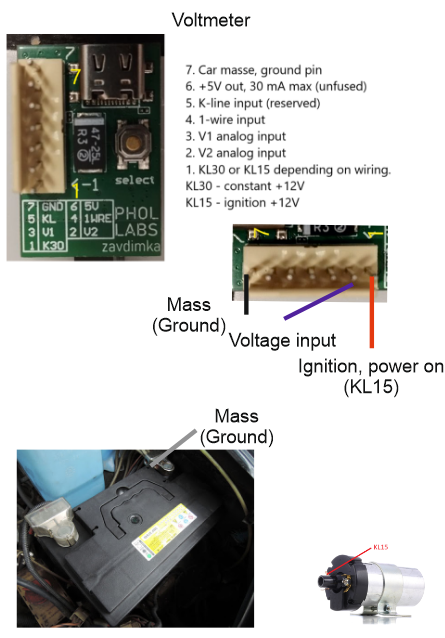
\includegraphics[width=.85\textwidth,height=.60\textheight,keepaspectratio]{figures/ivevo/image5.png}
\caption{Voltmeter diagram}
\end{figure}
\clearpage
\subsection{Gear indicator diagram}
\begin{figure}[H]
\centering
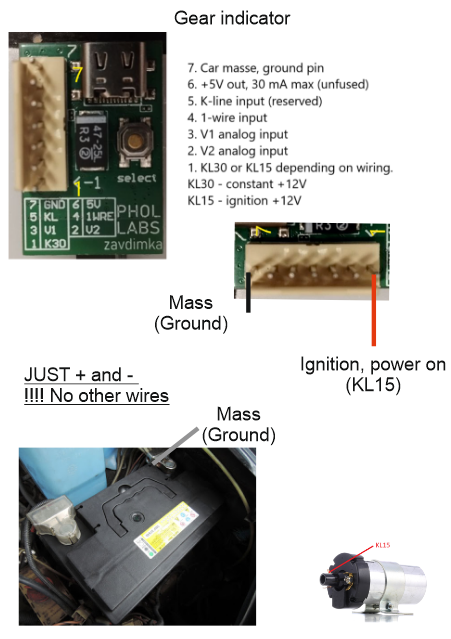
\includegraphics[width=.85\textwidth,height=.60\textheight,keepaspectratio]{figures/ivevo/image6.png}
\caption{Gear indicator diagram}
\end{figure}
\clearpage
\subsection{Barometer diagram}
\begin{figure}[H]
\centering
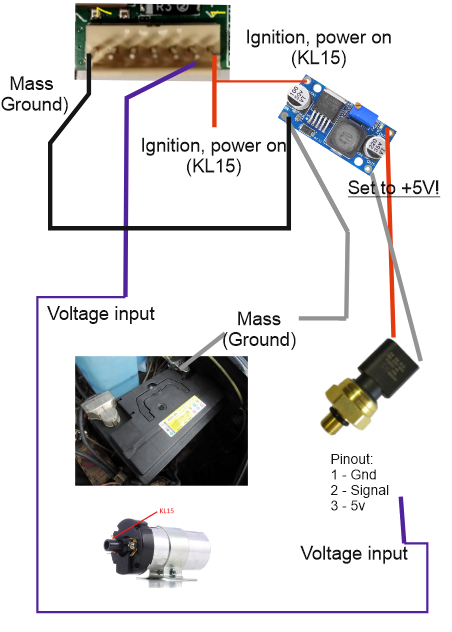
\includegraphics[width=.85\textwidth,height=.60\textheight,keepaspectratio]{figures/ivevo/image1.png}
\caption{Barometer diagram}
\end{figure}
\clearpage
\subsection{Thermometer diagram}
\begin{figure}[H]
\centering
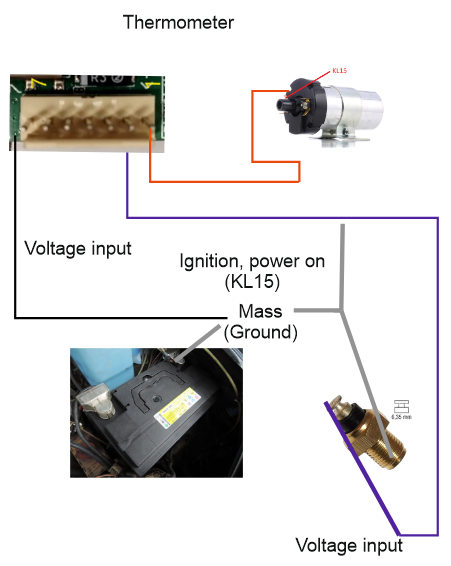
\includegraphics[width=.85\textwidth,height=.60\textheight,keepaspectratio]{figures/ivevo/image13.png}
\caption{Thermometer diagram}
\end{figure}
\clearpage
\subsection{Digital thermometer diagram}
\begin{figure}[H]
\centering
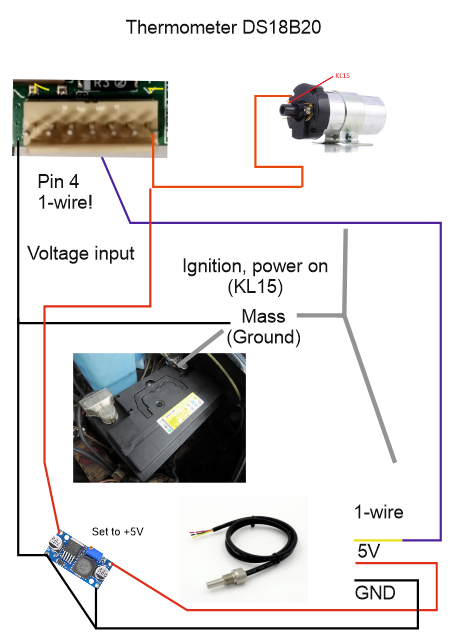
\includegraphics[width=.85\textwidth,height=.60\textheight,keepaspectratio]{figures/ivevo/image8.png}
\caption{Digital thermometer diagram}
\end{figure}
\clearpage
\subsection{Wideband lambda diagram}
\begin{figure}[H]
\centering
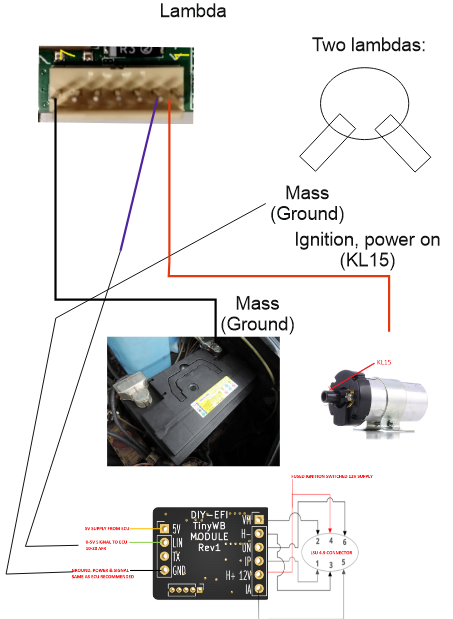
\includegraphics[width=.85\textwidth,height=.60\textheight,keepaspectratio]{figures/ivevo/image3.png}
\caption{Wideband lambda diagram}
\end{figure}
\clearpage
\subsection{Boost indicator diagram}
\begin{figure}[H]
\centering
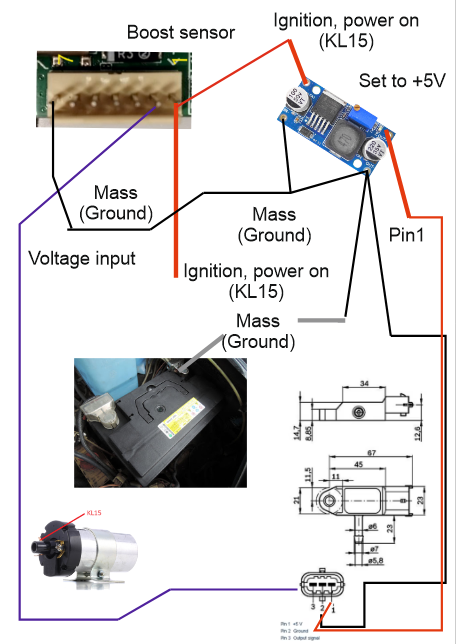
\includegraphics[width=.85\textwidth,height=.60\textheight,keepaspectratio]{figures/ivevo/image17.png}
\caption{Boost indicator diagram}
\end{figure}
